\documentclass[a4paper]{article}
\usepackage{float}
\usepackage{fullpage, amsmath, amssymb, verbatim} % Package to use full page
\usepackage{graphicx}
\usepackage{adjustbox}

\title{Deep Learning: Assignment Two}
\author{Aditi Nair (asn264) and Akash Shah (ass502)}
\date{April 4, 2017}
\begin{document}

\maketitle

\section{Batch Normalization}

\begin{enumerate}
\item{Let $x_1,...x_m$ be $m$ data points, and let $x_i^k$ be the $k$-th feature of the $i$-th data point. Then we define the mean $\mu_k$, of feature $x^k$, over a mini-batch as:
$$ \mu_k = \frac{1}{m} \sum_{i=1}^m x_i^k$$
and the variance $\sigma_k^2$ as:
$$ \sigma_k^2 = \frac{1}{m} \sum_{i=1}^m (x_i^k - \mu_k)^2$$

Now to normalize each feature $x^k$ (for $ 1 \leq k \leq n$) to have zero mean and unit standard deviation, we compute for each mini-batch value of that feature $x_i^k$, for $ 1 \leq i \leq m$: 
$$\hat{x}_i^k = \frac{x_i^k - \mu_k}{\sigma_k}$$

Then over all $\hat{x}_i^k$ per $k$, the expected value is $0$:
$$E[\hat{x}_1^k,...,\hat{x}_m^k] = \frac{1}{m} \sum_{i=1}^m \hat{x}_i^k = \frac{1}{m} \sum_{i=1}^m \frac{x_i^k - \mu_k}{\sigma_k} 
= \frac{1}{m} \frac{1}{\sigma_k} \sum_{i=1}^m (x_i^k - \mu_k) $$
$$ =  \frac{1}{m} \frac{1}{\sigma_k}  \Bigg[ \Bigg( \sum_{i=1}^m x_i^k \Bigg) - m \cdot \mu_k    \Bigg]
=  \frac{1}{m} \frac{1}{\sigma_k}  \Bigg[ \sum_{i=1}^m x_i^k  - \sum_{i=1}^m x_i^k  \Bigg] = 0$$
\newline
\newline
Then over all $\hat{x}_i^k$ per $k$, the variance is $1$ since:
$$Var[\hat{x}_1^k,...,\hat{x}_m^k] = \frac{1}{m}\sum_{i=1}^m (\hat{x}_i^k - \hat{\mu}_k)^2 = \frac{1}{m}\sum_{i=1}^m (\hat{x}_i^k - 0)^2 $$
$$ = \frac{1}{m}\sum_{i=1}^m (\hat{x}_i^k)^2 
=  \frac{1}{m}\sum_{i=1}^m \Big( \frac{x_i^k- \mu_k}{\sigma_k} \Big)^2 $$
$$ = \frac{1}{m}\sum_{i=1}^m  \frac{(x_i^k - \mu_k)^2}{\sigma_k^2} = \frac{1}{m \cdot \sigma_k^2} \sum_{i=1}^m  (x_i^k - \mu_k)^2$$
$$
= \frac{m}{m \cdot \sum_{i=1}^m (x_i^k - \mu_k)^2}  \sum_{i=1}^m  (x_i^k - \mu_k)^2 = 1
$$}

\item{ For $x_i^k$, the $k$-th feature of the $i$-th data point, the output of the BN module can be written as:
$$y_i^k = BN_{\gamma^k,\beta^k}(x_i^k) = \gamma^k \hat{x}_i^k + \beta^k $$
with
$$\hat{x_i}^k = \frac{x_i^k - \mu_k}{\sqrt{\sigma_k^2 + \epsilon}}$$
$\mu_k$ and $\sigma_k$ are defined as above. For numerical stability, the BN algorithm adds $\epsilon$ to $\sigma_k^2$ in the denominator of $\hat{x_i}^k$ before taking the square root.
\newline
\newline
\textbf{Now we write $\frac{\delta E}{\delta \gamma^k}$ in terms of $\frac{\delta E}{\delta y_i^k}$}:
\newline
\newline
$\gamma^k$ appears in the computation of each $y_i^k$ for $1 \leq i \leq m$. It follows that:
$$\frac{\delta E}{\delta \gamma^k} = \sum_{i=1}^m \frac{\delta E}{\delta y_i^k} \frac{\delta y_i^k}{\delta \gamma^k} $$
Then we notice that:
$$ \frac{\delta y_i^k}{\delta \gamma^k} =  \frac{\delta ( \gamma^k \hat{x}_i^k + \beta^k )}{\delta \gamma^k} = \hat{x_i}^k$$
Finally, we can write:
$$\frac{\delta E}{\delta \gamma^k} = \sum_{i=1}^m \frac{\delta E}{\delta y_i^k} \hat{x_i}^k $$
\newline
\newline
\textbf{Now we write $\frac{\delta E}{\delta \beta^k}$ in terms of $\frac{\delta E}{\delta y_i^k}$}:
\newline
\newline
$\beta^k$ appears in the computation of each $y_i^k$ for $1 \leq i \leq m$. It follows that:
$$\frac{\delta E}{\delta \beta^k} = \sum_{i=1}^m \frac{\delta E}{\delta y_i^k} \frac{\delta y_i^k}{\delta \beta^k} $$
Then we notice that:
$$ \frac{\delta y_i^k}{\delta \beta^k} =  \frac{\delta ( \gamma^k \hat{x}_i^k + \beta^k )}{\delta \beta^k} = 1$$
Finally, we can write:
$$\frac{\delta E}{\delta \beta^k} = \sum_{i=1}^m \frac{\delta E}{\delta y_i^k} $$

}


\end{enumerate}

\section{Convolution}

\begin{enumerate}
\item{In general, with a square input of length $I$, a square kernel of length $k$, zero padding of size $p$ on both sides, and a stride of $s$, we can calculate the output of convolution to be a square with length $(I-k+2p)/s + 1$. Assuming a stride of 1 and no zero padding, we will get a $3 \times 3$ matrix of $9$ values in the given problem.}
\item{
As stated in part 1, the output of forward propagating the image over the kernel will be a $3 \times 3$ matrix, whose values we can denote as $x_{i,j}$ for $i,j = 0,1,2$. In this problem, we consider the formulation of a discrete convolution where the kernel is not flipped, since both versions are equivalent when training a CNN. If we write the input image as $I_{i,j}$ for $i,j=0,\dots,4$ and the kernel as $k_{i,j}$ for $i,j = 0,1,2$, then we can express each value of the output in terms of the kernel and the input as follows:
$$
x_{i,j} = \sum_{m=0}^2 \sum_{n=0}^2 I_{i+m,j+n} \cdot k_{m,n}
$$
The result of this convolution is:

$$
\begin{bmatrix}
158 & 183 & 172 \\
229 & 237 & 238 \\
195 & 232 & 244 
\end{bmatrix}
$$

 }
\item{If we view our convolutional neural network as a feed-forward network, then our $5 \times 5$ input matrix would correspond to a layer in the feed-forward network with 25 units. The next layer would be our output from part 2, which we found has 9 units. Then, the weights connecting the two layers would be shared so that there are only 9 unique values of the weights, one for each kernel value. In this way, we can explicitly reconstruct the convolution formula above by viewing the value of a unit in the output layer as a sum of input units connected to that unit, scaled by the correspond weights of the connections. 
\newline
\newline
Now, let us consider the standard backpropagation method of a feed-forward network. Let $\delta_{i,j}^{l+1}$ for $i,j=0,1,2$ denote the gradients backpropagated from the layer above, and $\delta_{i,j}^{l}$ for $i,j=0,\dots,4$ denote the gradients backpropagated out of this input layer. By simply computing the backwards pass of the feed-forward network representing our CNN, we can see that the matrix of gradients out of this layer is equal to the convolution of the gradients from the layer above and kernel rotated $180^{o}$. The rotation of our initial kernel gives us the rotated kernel, $k^{*}$:
$$
\begin{bmatrix}
2 & 0 & 5 \\
9 & 7 & 2 \\
3 & 8 & 3 
\end{bmatrix}
$$
Now, the gradient matrix from the layer above will need zero-padding in order to apply a convolution properly, as our output needs to be a $5 \times 5$ matrix. By using padding of size 2 on each side, our gradient matrix from the layer above will be a $7 \times 7$ matrix, so the output of passing the $3 \times 3$ kernel over this gradient matrix will be the $5 \times 5$ gradient matrix backpropagated from the input layer.
Now using the same gradient formula as above, we have
$$
\delta_{i,j}^{l}= \sum_{m=0}^2 \sum_{n=0}^2 \delta_{i+m,j+n}^{l+1} \cdot k_{m,n}^{*}
$$
This convolution computation results in the following gradient matrix being backpropogated out of the input layer:
$$
\begin{bmatrix}
3 & 11 & 14 & 11 & 3 \\
5 & 20 & 32 & 27 & 12 \\
10 & 25 & 39 & 29 & 14 \\
7 & 14 & 25 & 18 & 11 \\
5 & 5 & 7 & 2 & 2 
\end{bmatrix}
$$
}
\end{enumerate}

\section{Variants of Pooling}
\begin{enumerate}
\item{Three types of pooling are max-pooling, average-pooling and L-P pooling. Max-pooling is implemented in different dimensions by the MaxPool1d, MaxPool2d and MaxPool3d classes in PyTorch. Average-pooling is implemented in different dimensions by the AvgPool1d, AvgPool2d, and AvgPool3d classes in PyTorch. L-P pooling is implemented in by the LPPool2d module in PyTorch. }
\item{  Now we define the mathematical forms of these pooling operations over a given set of input values $x_1,...,x_n$. 
Max pooling returns the maximum over all inputs:
$$MaxPool(x_1,...,x_n) = max( x_1, ...,x_n) $$
Average pooling computes the average of all the inputs:
$$AveragePool(x_1,...,x_n) = \frac{1}{n} \sum_{i=1}^n x_i$$
$L-p$ pooling computes the power-average of degree $p$ over the inputs:
$$LpPool(x_1,...,x_n) = \Bigg( \sum_{i=1}^n x_i^p \Bigg)^{\frac{1}{p}}$$

}
\item{ Max-pooling essentially applies a maximum function over (sometimes non-overlapping) regions of input matrices. For inputs with several layers of depth, max-pooling is generally applied separately for each layer's matrix. The pooling operation is used to reduce the size of the input matrices in each layer. Applying max-pooling will select only the maximum value in each region of the input matrix, discarding smaller values in each region. This can prevent overfitting by discarding information from the smaller values. In comparison, operations like average-pooling weigh all values in the region equally - and are therefore more conservative in discarding additional information. An average pooling operation in a region with many small values and one large value will have a relatively small output compared to the max pooling operation over the same region, which ignores the overall tendency of values in the region. Therefore the aggressive approach of the max pooling operation can be used as a regularizer. 
}
\end{enumerate}

\section{t-SNE}
\begin{enumerate}
\item{
The crowding problem refers to the tendency of dimensionality reduction techniques to crowd points of varying similarity close together.  Generally, SNE techniques model pairwise distances in high-dimensional space by a probability distribution $P$, and pairwise distances in the low-dimensional space by a probability distribution $Q$. In order to ensure that the low-dimensional representation is faithful to important properties of the original representation, SNE optimizes the KL-divergence between $P$ and $Q$ so that the pairwise distances in the low-dimensional space are as similar as possible to those in the original high-dimensional space. 
\newline
\newline
Maarten and Hinton (2008) provide the following examples to illustrate the crowding problem. Given a set of points which lie on a two-dimensional manifold in high-dimensional space, it is fairly straightforward to effectively describe their pairwise distances with a two-dimensional map. On the other hand, suppose these points lie on a higher-dimensional manifold - then it becomes much more difficult to model pairwise distances in two dimensions. Maarten and Hinton provide an example on a 10-dimensional manifold, where it is possible to have ten points which are mutually equidistant - this is clearly impossible to map into a two-dimensional space. 
\newline
\newline
More generally, the distribution of possible pairwise distances in the high-dimensional space is very different than the distribution of possible pairwise distances in the two-dimensional space. Consider a set of points in high-dimensional space which are uniformly distributed around a central point. As the distance of the points from the central point grows, the volume of space these points could occupy also grows. However in two dimensions there is less area to accommodate points which are moderately far from the center than there is to accommodate points which are near the center. Therefore, if we attempt to model small distances accurately in the two-dimensional space, we will be forced to place moderately large distances much further from the center point. Now, when trying to optimize the two-dimensional mapping, these too-far points will be pushed inward by the SNE objective function, effectively crowding all of the points together in the two-dimensional mapping.
\newline
\newline
t-SNE alleviates this by representing distances between points as probabilities using specific distributions. Distances in the high-dimensional spaces are converted to probabilities using a Gaussian distribution, whereas distances in the low-dimensional spaces are converted to probabilities using a distribution with a much heavier tail. This way, moderately far points are assigned larger distances in the lower-dimensional mapping compared to when the lower-dimensional distances are computed using a small-tailed distribution. Then the distances between pairs of moderately far points in higher dimensional space are closer to the distances between the same pairs of points in low dimensional space, and the SNE objective function will not push the low-dimensional representations closer together as much, ameliorating the crowding problem. 


}
\item{ Let 
$$C = KL(P || Q) = \sum_i \sum_j p_{ij} log\ \frac{p_{ij}}{q_{ij}} = \sum_i \sum_j p_{ij} log\ p_{ij} - p_{ij} log\ q_{ij}$$

We want to compute $\frac{\delta C }{\delta y_i}$. Note that $p_{ij}$ is constant with respect to $y_i$ but $q_{ij}$ is not. Specifically:
$$q_{ij} = \frac{ (1+ ||y_i - y_j ||^2)^{-1} }{\sum_{k \neq l} (1 + ||y_k - y_l ||^2)^{-1} }$$ 

Following the derivation of van der Maaten and Hinton, we define two intermediate values:
$$d_{ij} = ||y_i - y_j || $$
and 
$$Z = \sum_{k \neq l} (1 + d_{kl}^2)^{-1} $$

Now we can rewrite $q_{ij}$ as:
$$q_{ij} = \frac{(1+d_{ij}^2)^{-1} }{ \sum_{k \neq l} (1 + d_{kl}^2)^{-1} } = \frac{(1+d_{ij}^2)^{-1} }{  Z }$$

In the new notation, all terms are constant with respect to $y_i$ except $d_{ij}$ and $d_{ji}$ for all $j$. Now, we can compute the partial derivative $\frac{\delta C }{\delta y_i}$ in terms of the partial derivatives $\frac{\delta C }{\delta d_{ij}}$ and $\frac{\delta C }{\delta d_{ji}}$ for all $d_{ij}$ and $d_{ji}$. 
In particular, we notice that the terms $d_{ji}$ and $d_{ij}$ appears once each for all possible value of $j$. That is:
$$\frac{\delta C }{\delta y_i} = \sum_j  \frac{\delta C }{\delta d_{ij}} \frac{\delta d_{ij} }{\delta y_{i}} + \sum_j  \frac{\delta C }{\delta d_{ji}} \frac{\delta d_{ji} }{\delta y_{i}} $$

First, we compute $\frac{\delta d_{ij} }{\delta y_{i}}$. For $x,y \in \mathbb{R}^n$, notice that:
$$ ||x - y || =  \sqrt{ (x_{1}-y_{1})^2 + ... + (x_{n}-y_{n})^2  } $$

Then it follows that:
$$\frac{\delta \Big( ||x - y || \Big) }{\delta x} = \Big \langle \frac{\delta \Big( ||x - y || \Big) }{\delta x_1}, ..., \frac{\delta \Big( ||x - y || \Big) }{\delta x_n} \Big \rangle^T $$
$$ = \Big \langle \frac{2(x_1 - y_1) }{ 2 ||x-y|| }, ..., \frac{ 2(x_n - y_n)}{ 2 ||x-y|| } \Big \rangle^T $$
$$ = \frac{1}{||x-y||}\Big \langle x_1-y_1, ..., x_n - y_n \Big \rangle ^T = \frac{x-y}{||x-y||} $$

Since $d_{ij} = ||y_i - y_j || $, it follows that:
$$\frac{\delta d_{ij}  }{\delta y_i} = \frac{\delta \Big( ||y_i - y_j || \Big) }{\delta y_i} = \frac{y_i - y_j}{ ||y_i - y_j ||} $$

Moreover since $d_{ji} = ||y_j - y_i || = ||y_i - y_j ||  = d_{ij} $, we can say that: 
$$\frac{\delta d_{ji}  }{\delta y_i} = \frac{y_i - y_j}{ ||y_i - y_j ||} $$

Finally:
$$\frac{\delta C }{\delta y_i} = \sum_j  \frac{\delta C }{\delta d_{ij}} \frac{y_i - y_j}{ ||y_i - y_j ||} + \sum_j  \frac{\delta C }{\delta d_{ji}} \frac{y_i - y_j}{ ||y_i - y_j ||} $$
$$ =  \sum_j  \Big( \frac{\delta C }{\delta d_{ij}} +  \frac{\delta C }{\delta d_{ji}} \Big) \frac{y_i - y_j}{ ||y_i - y_j ||} =  2 \sum_j  \frac{\delta C }{\delta d_{ij}}  \frac{y_i - y_j}{ ||y_i - y_j ||} = 2 \sum_j  \frac{\delta C }{\delta d_{ij}}  \frac{y_i - y_j}{ d_{ij} } $$

Next, we need to compute $ \frac{\delta C }{\delta d_{ij}} $. Recall that: 
$$C = \sum_i \sum_j p_{ij} log\ p_{ij} - p_{ij} log\ q_{ij}$$
and only $q_{ij}$ is non-constant with respect to $d_{ij}$. 

Therefore: 
$$\frac{ \delta C }{\delta d_{ij} } = \frac{ \delta \Big( \sum_i \sum_j p_{ij} log\ p_{ij} - p_{ij} log\ q_{ij} \Big) }{\delta d_{ij} } $$
$$ = \frac{ - \delta \Big( \sum_i \sum_j p_{ij} log\ q_{ij} \Big) }{\delta d_{ij} } $$

When optimizing t-SNE, we define $p_{ii} = q_{ii} = 0$ for all $i$. Then we can say:
$$\frac{ \delta C }{\delta d_{ij} } = \frac{ - \delta \Big( \sum_{k \neq l} p_{kl} log\ q_{kl} \Big) }{\delta d_{ij} } $$

Following, the derivation of van der Maaten and Hinton, we observe that:
$$log\ q_{kl} = log \frac{q_{kl} Z}{Z} = log\ q_{kl} Z - log Z $$

It follows that:
$$\frac{ \delta C }{\delta d_{ij} } = \frac{ - \delta \Big( \sum_{k \neq l} p_{kl} (log\ q_{kl} Z - log Z) \Big) }{\delta d_{ij} } $$

Notice that $q_{kl}$ and $Z$ are non-constant with respect to $d_{ij}$ and that:
$$q_{kl} Z =  \frac{(1+d_{kl}^2)^{-1} }{  Z } Z = (1+d_{kl}^2)^{-1} $$

Then we can compute $\frac{ \delta C }{\delta d_{ij} }$ as:
$$\frac{ \delta C }{\delta d_{ij} } = - \sum_{k \neq l} p_{kl} \Big( \frac{1}{q_{kl} Z }  \frac{\delta (1+d_{kl}^2)^{-1}  }{\delta d_{ij}} - \frac{1}{Z} \frac{\delta Z }{\delta d_{ij}} \Big) $$

Now we notice that $\frac{\delta (1+d_{kl}^2)^{-1} }{\delta d_{ij}}$ is $0$ unless $k=i$ and $l=j$. Then we can write:
$$\frac{ \delta C }{\delta d_{ij} } =  \frac{ - p_{ij} }{q_{ij} Z } \cdot -  (1+d_{ij}^2)^{-2} \cdot 2 d_{ij} - \sum_{k \neq l} - p_{kl} \frac{1}{Z} \cdot -(1 + d_{ij}^2)^{-2} \cdot 2 d_{ij}$$
$$ =  \frac{  2 p_{ij} }{q_{ij} Z } \cdot (1+d_{ij}^2)^{-2} \cdot d_{ij} - 2 \sum_{k \neq l}  \frac{ p_{kl}}{Z} \cdot (1 + d_{ij}^2)^{-2} d_{ij} $$

Since $q_{ij} Z = (1+d_{ij}^2)^{-1}$ we can simplify the left summand further.
$$\frac{ \delta C }{\delta d_{ij} }  =   2 p_{ij} \cdot (1+d_{ij}^2)^{-1} \cdot d_{ij} - 2 \sum_{k \neq l}  \frac{ p_{kl}}{Z} \cdot (1 + d_{ij}^2)^{-2} d_{ij} $$
$$ =   2 p_{ij} \cdot (1+d_{ij}^2)^{-1} \cdot d_{ij} - \frac{2}{Z} \sum_{k \neq l}  p_{kl} \cdot (1 + d_{ij}^2)^{-2} d_{ij} $$
Since $\sum_{k \neq l} p_{kl} = 1$:
$$\frac{ \delta C }{\delta d_{ij} }  =   2 p_{ij}  (1+d_{ij}^2)^{-1}  d_{ij} - \frac{2}{Z} (1 + d_{ij}^2)^{-2} d_{ij} $$
Since $q_{ij} = \frac{(1+d_{ij}^2)^{-1} }{  Z }$, we can simplify the right summand as:
$$\frac{ \delta C }{\delta d_{ij} }  =   2 p_{ij}  (1+d_{ij}^2)^{-1}  d_{ij} - 2 q_{ij} (1 + d_{ij}^2)^{-1} d_{ij} $$
$$ = 2 (p_{ij} - q_{ij}) (1+d_{ij}^2)^{-1}  d_{ij} $$

Now we can substitute this into our expression for $\frac{\delta C }{\delta y_i}$:
$$\frac{\delta C }{\delta y_i} = 2 \sum_j  \frac{\delta C }{\delta d_{ij}}  \frac{y_i - y_j}{ d_{ij} } = 2 \sum_j  \Big( 2 (p_{ij} - q_{ij}) (1+d_{ij}^2)^{-1}  d_{ij}  \Big) \frac{y_i - y_j}{ d_{ij} }$$
$$\frac{\delta C }{\delta y_i}  = 4 \sum_j  (p_{ij} - q_{ij}) (1+d_{ij}^2)^{-1} (y_i - y_j)$$

}
\end{enumerate}

\section{Sentence Classification}


\subsection{ConvNet}

\begin{enumerate}

\item{
Given a sentence of 10 words, each word has a trained word embedding vector of dimension 300. Thus, we can construct an input matrix, $I \in \mathbb{R}^{10 \times 300}$, where the $i$-th row is the word embedding of the $i$-th word in the sentence. Each filter will be a matrix with length equal to the word embedding size, but can have a varied width (or filter size). If we have 5 filters, with filter sizes of 2, 3, 4, 5, and 6, and each with a length of 300, then by passing each filter over the input matrix and performing convolutions, we will obtain a hidden feature vector for each filter. For a filter with size $k$, the hidden feature vector will have a length of $10-k+1$, so we will obtain 5 feature vectors with lengths 9, 8, 7, 6, and 5. These feature vectors will then be passed into a ReLU layer, which applies the non-linearity $ReLU(x) = max(x,0)$ element-wise to the input vectors. Since the ReLU layer is applied element-wise, the outputs have the exact same dimensions as the inputs, so we will still have 5 feature vectors with lengths 9, 8, 7, 6, and 5.
\\\\By applying max-pooling to each feature vector, each of the 5 vectors will be reduced to a scalar value, and concatenating them will result in a vector of length 5, $f \in \mathbb{R}^5$. We can then pass this vector of length 5 into a fully-connected layer with 5 input units and 3 output units, which has a corresponding weight matrix $V \in \mathbb{R}^{3 \times 5}$. The output of this fully-connected layer will be a vector with 3 scores, one for each class, ie $s \in \mathbb{R}^{3}$ which is computed as $s = Vf$. Finally, we pass the vector of scores into a softmax function to obtain a probability for each of the 3 classes. 
}

\item{
In a single-layer CNN such as the one described above, small filter sizes can be viewed as small n-gram featurizations of the input but in a dense and distributed vector space, while large filter sizes would be larger n-grams. However, in a deep CNN, even small filter sizes can result in learnings of language dependencies across higher order n-grams because adjacent k-grams that did not overlap during the convolution in the current layer will then be convoluted over together in the next layer. 
\\\\
Our approach in choosing filter sizes would be to have multiple filters of various sizes so that different featurizations can be learned by the CNN. To select filter sizes, apply convolution filters which are as tall as the value of $n$-grams which you think will be helpful for the classification task. Next, the model applies max-pooling (and a non-linearity) to the output of each filter, followed by a fully-connected layer and a soft-max function. Therefore, if a single convolution filter is more or less important than others, then the column of the fully-connected layer's weight matrix which uses the output of max-pooling on that filter will be given larger or smaller weights by a successful optimization algorithm.
}
\end{enumerate}

\subsection{RNN}

\begin{enumerate}

\item{ Let $w_1,...,w_T$ be an input sentence, and let $x_1,...x_T$ be the corresponding word embeddings. Let $f$ represent a recursive neural net which computes the hidden state $h_t$ of the network at time $t$. At time $t$ in a simple RNN, we use the hidden state of the RNN at time $t-1$, $h_{t-1}$, and the word embedding for the current input word, $x_t$, to generate the hidden state vector at time $t$: 
$$h_t = f(x_t, h_{t-1}) $$ 
(Usually we set $h_0 = \vec{0}$.) Now, we can recursively apply $f$ to the sequence $x_1,...x_T$ to get $h_T$, the hidden state at the final time step, which will summarize the input of the entire sentence.}

\item{ Each word in the sentence will correspond to a word embedding vector $x_t \in \mathbb{R}^{300}$. We will initialize $h_0 = \vec{0}$ with length 50, since we want the sentence to be summarized by a vector of length 50. Additionally, we will have two weight matrices: $U \in \mathbb{R}^{50 \times 300}$ and $W \in \mathbb{R}^{50 \times 50}$. Finally, we will have a bias vector: $b \in \mathbb{R}^{50}$.
\\\\
Then, we can define our simple RNN as:
$$
h_t = f(x_t,h_{t-1}) = \tanh (Ux_t + Wh_{t-1} + b)
$$
The matrix product $Ux_t$ will transform the input word vector of length 300 into a vector of length 50, while the matrix product $Wh_{t-1}$ takes an input hidden state vector of length 50 and outputs a vector that still has a length of 50. Thus, the vector addition $Ux_t + Wh_{t-1} + b$ adds three vectors each of length 50. Finally, the $\tanh$ is applied element-wise, so our output hidden state vector $h_t$ is a vector of length 50.
\\\\
Given a sentence of length 10, after the last input word has been fed into the RNN, we will obtain $h_{10} \in \mathbb{R}^{50}$, which summarizes our sentence. Then, we can feed this vector into a fully-connected layer with 50 input units and 4 output units. Let $V \in \mathbb{R}^{4 \times 50}.$ Then the fully-connected layer computes:
$$s = V h_{10} $$
Now $s$, the output of the fully-connected layer, is in $\mathbb{R}^4$, containing a score for each of the four classes. Finally, we can feed this vector into a soft-max function which will give us 4 probabilities, one for each class.  
}

\end{enumerate}


\subsection{Extra credit experiments of fastText}
fastText is a popular and often-effective model for sentence classification. Let $w_1,...,w_n$ be an input sentence that we would like to classify into binary classes, $\{0,1\}$. Let $\tilde{x}_1,...,\tilde{x}_N \in \mathbb{R}^V$ be n-gram features corresponding to the input sentence, where $V$ is the total number of features and $N$ is the total number of corresponding n-grams that appear in $w_1,...,w_n$. Let $E \in \mathbb{R}^{d \times V}$ be an embedding matrix and define:
$$x_i = E \tilde{x}_i $$
Now $x_1,...,x_N \in \mathbb{R}^{d}$ are word embeddings corresponding to the n-gram features of the input sentence. Then compute:
$$\mu = \frac{1}{n} \sum_{i=1}^n x_i $$
Now we pass the average of the word embeddings through a linear classifier to compute a score $p = p(y=1 | w_1,...,w_n)$:
$$ p = W \mu + b $$
Finally, we train the model to maximize the probability of the correct class, or equivalently, to minimize the negative log-likelihood of the correct class. 
\newline
\newline
There are two main advantages to the fastText model - in addition to strong empirical performance. The first is that it is a fairly straightforward and efficient model, and can have fewer parameters to train compared to a large RNN or ConvNet model. Then second is that, unlike an ConvNet, the fastText model can accept variable-length input. Though many fastText implements only consider fixed windows of inputs, this is not necessary from a mathematical standpoint since we average the embedding vectors of the input sequence.
\newline
\newline
Unlike ConvNet and RNN, fastText takes a bag-of-words/bag-of-n-grams approach to word order, since it averages the embeddings corresponding to all of the n-grams and tokens of the input sentence. In contrast, RNNs traverse input sequences in order, and are therefore attentive to word order. Similarly, ConvNets used for natural language tasks process input sentences by stacking word embedding vectors together in an ordered manner before applying convolution, pooling and fully-connected layers, which is also attentive to word order. With fastText, in order to capture longer-term relationships between far-apart tokens, our best approach is to consider larger-sized n-gram features. However, this can become problematic. As the size of the n-gram grows, the number of possible n-grams also grows and we begin to encounter issues of sparsity, where we have little data associated with many of the large n-grams. This increases our model complexity in a manner that is, at best, prone to overfitting and, at worst, uninformative. For a language modeling task, this can be especially challenging since word order - and specifically long-term dependencies - can indicate crucial information. 
\newline
\newline
We trained a simple fastText language model on Penn Treebank data with the default parameters found in Facebook's fastText implementation for five epochs and a window size of 20. Since the fastText package computes accuracy and not perplexity, we cite this below:

\begin{center}
\begin{tabular}{ |c|c| } 
 \hline
 Validation Accuracy & 8.12 \% \\ \hline
 Test Accuracy & 8.17 \% \\
 \hline
\end{tabular}
\end{center}

Below, we give some examples of how fastText predicts the missing next word in a sentence compared to what the actual word is:

\begin{center}
\begin{tabular}{ |c|c|c|} 
 \hline
Input & Predicted & Actual \\ \hline
consumers may want to move their telephones a little closer to the tv \\ set UNK UNK watching abc 's monday & night & UNK \\ \hline
may want to move their telephones a little closer to the tv set UNK \\ UNK watching abc 's monday night & football & UNK \\ \hline
want to move their telephones a little closer to the tv set UNK \\ UNK watching abc 's monday night football & can & UNK \\ \hline
\end{tabular}
\end{center}

From these experiments, it is clear that we have a very poor language model, since it simply guesses a somewhat common token in the vocabulary for each input. These results also suggest that the model can be insensitive to word order and content, since it guesses the same value for each input even though every pair of inputs differ in at least two tokens. Finally, however, it is worth noting that this was a somewhat small model which was not trained for very long, so we should not make definitive claims about its potential.

\subsection{Extra credit question}
Here we propose a new neural architecture for sentence classification. Let $f$ represent a recursive neural net which computes the hidden state $h_t$ of the network at time $t$. Let $w_t$ be the $t$-th word in the input sentence $(w_1,...w_T)$ and $\tilde{x_t}$ be its corresponding one-hot vector. The we define $x_t$ as:
$$x_t = E \tilde{x_t} $$
where $E \in \mathbb{R}^{d \times V}$ is the embedding matrix. $V$ is the vocabulary size and length of $\tilde{x_t}$, and $x_t \in \mathbb{R}^d$ is the word embedding corresponding to the input token at $w_t$. 
\newline
\newline
Then we can set $h_0 = \vec{0}$ and compute the hidden state at time $t$ as:
$$h_t = f(x_t, h_{t-1}) $$ 
We can recursively compute $h_T$ which will contain a summary of the entire input sentence.
\newline
\newline
Using this RNN we can compute the hidden states $h_1,...,h_{T}$ for each time-step in the input sentence. Next, we line up the vectors so that we have a matrix which has height $T$ and width $d$. 
\newline
\newline
Now we can pass this matrix as input to a convolutional neural network. Specifically, apply several convolution filters of width $d$ to the input matrix. Apply max-pooling over the vector resulting from each convolution. Concatenate the results - the current vector will be as long as the number of convolution filters. Then apply an element-wise non-linearity and pass through a soft-max layer. 
\newline
\newline
This network is a hybrid RNN-CNN network. Traditional RNNs often struggle to appropriately weigh and ``remember" long-term information over many time-steps. Though alternative recurrent modules (like GRUs and LSTMs) and architectures (like attention and memory networks) have been proposed to alleviate this problem, in practice these can have limited success. This hybrid network could potentially alleviate this problem since we incorporate the hidden vectors from each time step in the matrix that is passed as input to the CNN. 
\newline
\newline
Additionally, the RNN is also helpful since it allows us to incorporate location-invariant information about word and phrase meaning in the input. Since RNNs are computed recursively, information that is learned in the beginning of an input sequence can also be applied at the end of the sequence. The CNN does not do this as naturally, since it must first find the right convolution and pooling filters to diffuse information learned across different regions of the input space. Therefore, by using $h_1,...h_T$ for the input matrix to the CNN we can incorporate location-invariant information from the input sentence more easily.
\newline
\newline
Finally, a major downside of CNNs in language applications is that they can only accept fixed-size inputs. Indeed, even in this model, we must fix the size of the input matrix to the CNN and then either clip or pad the sequences of hidden state vectors as necessary. Clipping the sequence of hidden state vectors is especially damaging since it forces us to throw out valuable information from the input sentence. However, since RNNs recursively compute the hidden state at time $t$, $h_t$ contains information from $w_t$ as well as from $w_1, ... w_{t-1}$. Therefore, even if we are forced to throw out some $h_t$ vectors, by keeping the ``older" $h_t$ vectors, we can ensure that some of the information from the ``earlier" vectors is still retained by the network. 
\newline
\newline

\section{Language Modeling}

We used RNNs to develop language models for the Penn Treebank (PTB) and Gutenberg datasets. For each dataset, we discuss the tuning process for model hyper-parameters, and also provide quantitative and qualitative analysis of the results. For both datasets, we relied on a greedy procedure for hyper-parameter selection: once a certain hyper-parameter was shown to produce a lower perplexity on our validation set, that hyper-parameter was generally included in all subsequent models. 

\section*{Penn Treebank Language Model}
Initially, we trained a baseline model using the default hyper-parameters of the provided starter code. We detail these hyper-parameters below, since all subsequent models are loosely based off of these. 

\subsection*{Model Description and Hyper-parameter Selection}

\begin{table}[h]
\centering
\begin{tabular}{|c | c|} 
 \hline
RNN Cell & LSTM\\ \hline
Optimizer & SGD w/ gradient clipping \\ \hline
Learning Rate & 20 \\ \hline
Epochs & 6\\ \hline
Layers & 1\\ \hline
Embedding Dim. & 50\\ \hline
Num. Hidden Units & 50\\ \hline
Parameter Init. & Random Uniform from [0,0.1]\\ \hline
Vocabulary size & 10k\\ \hline
Shuffle after epoch & No \\ \hline
\textbf{Validation Perplexity} &\textbf{147.16} \\ \hline
\end{tabular}
\caption{PTB Baseline Hyper-parameters and Result}
\label{table:1}
\end{table}

Next, we explored a range of hyper-parameters to improve the model perplexity. Note that we did not modify the vocabulary size in these experiments since the provided data had already processed the data to a fixed vocabulary size of 10,000, with all out-of-vocabulary tokens replaced with an ``unk" token. 
\newline
\newline
First, we added a second layer to the baseline model. This improved the validation perplexity from 147.16 to 137.56. (Since this parameter improved our validation perplexity, it is included in all subsequent models.) Next we experimented independently with increasing the embedding dimension and the number of hidden units in each layer from 50 to 100. Increasing only the embedding dimension only decreased the validation perplexity from 137.56 to 137.44. Increasing only the hidden state decreased the validation perplexity from 137.56 to 122.83. Increasing both values from 50 to 100 improved the validation perplexity to 122.44. Next, we allowed the model to train for 15 full epochs, giving us a validation perplexity of 122.44. Finally, increasing the number of hidden units to 200 reduced the validation perplexity to 119.59, and subsequently increasing the embedding dimension reduced the validation perplexity to 118.79.
\newline
\newline
At this stage, we summarize our Intermediate Model as:

\begin{table}[h!]
\centering
\begin{tabular}{|c | c|} 
 \hline
RNN Cell & LSTM\\ \hline
Optimizer & SGD w/ gradient clipping \\ \hline
Epochs & 15\\ \hline
Layers & 2\\ \hline
Embedding Dim. & 200\\ \hline
Num. Hidden Units & 200\\ \hline
Parameter Init. & Random Uniform from [0,0.1]\\ \hline
Vocabulary size & 10k\\ \hline
Shuffle after epoch & No \\ \hline
\textbf{Validation Perplexity} &\textbf{118.79} \\ \hline
\end{tabular}
\caption{PTB Intermediate Model Hyper-parameters and Result}
\label{table:1}
\end{table}

From these experiments, we conclude that increasing the number of layers, the embedding dimension and the number of hidden units can have a significant impact on perplexity. By modifying these parameters alone, and by allowing our model to train longer, we reduced our perplexity from 145.28 to 118.79.
\newline
\newline
Next, we experimented with different recurrent units for the network, and different gradient descent procedures for training the network. First, we used GRU cells rather than the default LSTM cells. This resulted in an increase in validation perplexity to 309.98. GRU cells have been known to train more slowly than LSTM cells; we attempted to ``hack" this property by simply increasing the learning rate rather than training the model for longer. However, using GRU cells with a learning rate of 50 further increased our validation perplexity to 661.69. Finally, given our poor results, and since GRUs and LSTMs generally often have comparable performance, we chose to simply use LSTMs.
\newline
\newline
To this point, most of our models had been trained using an initial learning rate of 20, which was annealed over time by a factor of 4 when subsequent epochs showed increased perplexity on the validation set. Next, we explored different optimization methods. In addition to the Adam optimization algorithm, we tested different parametrizations for SGD with Nesterov's Accelerated Gradient (NAG) method. We present the results of these experiments below.

\begin{table}[h!]
\centering
\begin{tabular}{|c | c|} 
 \hline
Optimization Method & Validation Perplexity \\ \hline \hline
Adam with Learning Rate 0.001 & 199.86 \\ \hline
SGD with NAG: Learning Rate 0.1 and Momentum Coeff. 0.9 & 140.07\\ \hline
SGD with NAG: Learning Rate 0.05 and Momentum Coeff. 0.5 & 317.17 \\ \hline
SGD with NAG: Learning Rate 0.1 and Momentum Coeff. 0.5 &215.71 \\ \hline
\end{tabular}
\caption{Experiments with Optimizers}
\label{table:1}
\end{table}
Clearly, these results were worse than our previous models. Though we were not convinced that modifying the optimizer \textit{wasn't} a useful approach, it was too time-consuming to continuing exploring the parameters for more optimizers, since at this point our model was fairly large and required about 2 hours to train for 15 epochs. 
\newline
\newline
In our final experiments, we experimented with regularizing our model, shuffling the training data, and simply making our model bigger. Below, we present the results of applying dropout - which is a form of regularization - on our models. Both experiments were an improvement over our best model thus far, but the model with dropout ``keep" probability 0.3 had a smaller perplexity. Since this model had the lowest perplexity, we included dropout with probability 0.3 in all subsequent experiments.

\begin{table}[h!]
\centering
\begin{tabular}{|c | c|} 
 \hline
Dropout ``Keep" Probability & Validation Perplexity \\ \hline \hline
0.5 & 116.22 \\ \hline
0.3 & 114.54\\ \hline
\end{tabular}
\caption{Experiments with Dropout}
\label{table:1}
\end{table}

Next, rather than shuffle all of the training data, we decided to only shuffle the batches of data. Though this did not have the full effect of shuffling the training data, it was more appropriate given the structure of the code. In the provided code, the entire training file is treated as a single document. Therefore, consecutive sentences on separate lines of the file are modeled as having a sequential relationship. For this reason, it was inappropriate to shuffle the lines of the training file, since this fundamentally changes the training corpus, and we can no longer directly compare models. Then the alternative was to read all possible sequences within the corpus into memory, then shuffle the sequences before each epoch, and then process them in batches according to the optimization algorithm. This was likely to slow our training procedure significantly, so we did not pursue this. Surprisingly, using shuffled batches of training data increased the validation perplexity to 122.71, so we did not use this in subsequent experiments.
\newline
\newline
Finally, out of curiosity, we tried train to significantly larger models. In our original experiments, we observed that increasing the number of layers, the embedding dimension and the number of hidden units had the most effect on our models, so we wondered whether increasing these values more would further reduce our perplexity. As we show below, these experiments did not improve our model perplexity:
\begin{center}
\begin{tabular}{|c | c | c | c |} 
\hline
Layers & Embedding Dim. & Num. Hidden Units & Validation Perplexity \\ \hline \hline
3 & 200 & 200 & 121.16 \\ \hline
3 & 300 & 300 & 122.93 \\ \hline
\end{tabular}
\end{center}

Below, we describe the final hyper-parameters of the model with the lowest validation perplexity, and additionally report its test perplexity:
\begin{table}[H]
\centering
\begin{tabular}{|c | c|} 
 \hline
RNN Cell & LSTM\\ \hline
Optimizer & SGD w/ gradient clipping \\ \hline
Epochs & 15\\ \hline
Layers & 2\\ \hline
Embedding Dim. & 200\\ \hline
Num. Hidden Units & 200\\ \hline
Parameter Init. & Random Uniform from [0,0.1]\\ \hline
Vocabulary size & 10k\\ \hline
Shuffle after epoch & No \\ \hline
Dropout Keep Prob. & 0.3 \\ \hline
\textbf{Validation Perplexity} &\textbf{114.54} \\ \hline
\textbf{Test Perplexity} &\textbf{108.93} \\ \hline
\end{tabular}
\caption{PTB Final Model Hyper-parameters and Result}
\label{table:1}
\end{table}

Now, we provide examples of text generated by our models. Below, we provide samples from our baseline model:
\begin{table}[h]
\centering
\begin{tabular}{|c|} \hline
m. quayle director of the government close $\langle$ eos $\rangle$ \\ \hline
the dollar stood up N points in the second constitution $\langle$ eos $\rangle$ \\ \hline 
the tokyo hills general had in the shield interest would be \\ $\langle$ unk $\rangle$ and can oppose a broad version of the river $\langle$ eos $\rangle$ \\ \hline
by mr. $\langle$ unk $\rangle$ 's house is $\langle$ unk $\rangle$  \\ \hline
\end{tabular}
\caption{Language samples for PTB Baseline}
\label{table:1}
\end{table}

From these examples, we can observe that the model emits a fair number of $\langle$ unk $\rangle$ tokens. We can also observe that the model is fairly adept at generating reasonable phrases like: ``director of the government", ``the dollar stood up N points" and ``oppose a broad version of the". (`N' is how numbers are encoded and decoded by the model.) This suggests that our model has converged to some reasonable understanding of when certain tokens are used, and in what local context. In general, these appear to be phrases that could occur reasonably often in the Wall Street Journal, the source of the PTB Corpus. However, almost uniformly, the examples shown above lack any overall meaning. That is, far-apart tokens generated by the model lack cohesion - the model lacks effective long-term dependencies between these tokens.
\newline
\newline
Next, we consider text generated by our final model:

\begin{table}[h]
\centering
\begin{tabular}{|c|} \hline
paramount communications said net rose N N $\langle$ eos $\rangle$ \\ \hline
it involved in federal court in dallas for december delivery said it agreed \\
to cut its barriers to shareholders $\langle$ eos $\rangle$ \\ \hline
although a \$ N million to tax reserves is already capable of punts a \\ 
tax-loss set around the start of meredith 's third-quarter charge \\
for a doubling in the next three quarters $\langle$ eos $\rangle$  \\ \hline
\end{tabular}
\caption{Language samples for PTB Final Model}
\label{table:1}
\end{table}

Surprisingly, though the perplexity of this model is significantly lower than the baseline, the language samples it generated do not seem to be particularly more coherent. In language samples generated by the final model, we observe that the subject is quite consistently related to finance and business, the main focus of the Wall Street Journal. The first example - ``paramount communications said net rose N N" - is a sensible and meaningful, but short, sentence. However, the next two examples, which are at least twice as long, are not so meaningful. In both sentences, though there is some local coherence between words in the form of meaningful phrases - ``involved in federal court in dallas", ``agreed to cut its barriers to shareholders", ``doubling in the next three quarters" - the sentences as a whole lack meaning, perhaps again because the model lacks effective long-term dependencies between tokens. That is to say, the tokens generated later in the sentences are not sufficiently conditioned on those generated very early in the sentence, and therefore are not necessarily relevant to them.



\section*{Gutenberg Language Model}
For our analysis of a second dataset, we used the Gutenberg data provided. However, since this dataset was 3 times as large as the Penn Treebank data, we downsampled the dataset to $\sim$800K training examples from $\sim$2.5M training examples. As with the Penn Treebank data, our exploration process was done in a greedy manner - once we found an optimal parameter value for a specific parameter, that value was used in subsequent experiments while exploring other parameters. Our baseline model used the default parameters of the provided starter code, and are summarized below:

\begin{table}[H]
\centering
\begin{tabular}{|c | c|} 
 \hline
RNN Cell & LSTM\\ \hline
Optimizer & SGD w/ gradient clipping \\ \hline
Learning Rate & 20 \\ \hline
Learning Rate Decay & 4 \\ \hline
Epochs & 15\\ \hline
Layers & 1\\ \hline
Embedding Dim. & 50\\ \hline
Num. Hidden Units & 50\\ \hline
Parameter Init. & Random Uniform from [0,0.1]\\ \hline
Vocabulary size & 10k\\ \hline
Shuffle after epoch & No \\ \hline
\textbf{Validation Perplexity} &\textbf{104.86} \\ \hline
\end{tabular}
\caption{Gutenberg Baseline Hyper-parameters and Result}
\label{table:1}
\end{table}

\subsection*{Model Description and Hyper-parameter Selection}
In our parameter exploration process, we first modified the word embedding and hidden state sizes. Since both dimensions were initially 50, we tried setting each to 25 and 100, while the other was held constant at 50. Of these, having an embedding size of 25 while keeping hidden state size at 50 improved validation perplexity to 104.04, while having a hidden state size of 100 while keeping the embedding size at 50 improved the perplexity to 100.06. Since increasing the hidden state size to 100 resulted in the best improvement, we tried varying the embedding dimension while keeping the hidden state size at 100. Embedding dimensions of 25 and 100 were tested, but neither decreased the validation perplexity any further. Thus, the optimal parameters thus far were a hidden state size of 100 and an embedding size of 50. 
\newline
\newline
Next, we tried changing the learning rate and learning rate decay, with the hope that a learning rate that decays less quickly might learn better in later epochs. The default learning rate was 20 and the default decay was 4, so we tried changing the decay to 2 instead of 4, and then also tried changing both the learning rate to 10 and the decay to 2. However, neither modification improved the model. We also tried changing the LSTM cells to GRU cells instead, however this did not improve the model which was expected. Since GRU cells have less parameters than LSTM cells, they often can converge more quickly than LSTM cells but rarely outperform LSTM models that have been run for the same number of epochs.
\newline
\newline
Next we experimented with weight initialization in the model. The default behavior were weights sampled from a Uniform distribution in [0,0.1]. We tried using a Normal distribution instead of Uniform as this often increases performance empirically. We tried a Normal distribution with mean 0 and standard deviation 0.1 which improved the validation perplexity to 99.21. We also tried a Normal distribution with mean 0 and standard deviation of 0.01, however this did not work as well as a standard deviation of 0.1. Then, we tried increasing the depth of the model by increasing the number of layers from 1 to 2. This improved the validation perplexity to 98.81. Then, we tried shuffling the batches before each epoch which further improved the perplexity to 97.75.
\newline
\newline
The baseline model used Stochastic Gradient Descent as the optimization method. We tried using the Adam optimizer instead, with a learning rate of .001 which is standard for the Adam optimizer. However, this made the perplexity considerably worse as it was around 124, so it seemed that the Adam optimizer did not work well given the current parameter values or the dataset. Finally, we tried adding dropout on the vertical connections between the layers. We tried dropout probabilities of 0.5 and 0.3, and both significantly improved the validation perplexity of our model. Dropout with p=0.5 improved the validation perplexity to 96.2, while dropout with p=0.3 improved it even further to 94.9.
\newline
\newline
Since models with smaller vocabulary sizes naturally have a smaller perplexity, we did not experiment with the vocabulary size until the very end. We tried having vocabulary sizes of 5,000 and 15,000 with the current version of the best model, which until then had a vocabulary size of 10,000. Since perplexity could not be used to compare them, we generated samples from all three models and used them in a qualitative analysis.
Below are samples for each version that we thought were representative of the model:

\begin{table}[h]
\centering
\begin{tabular}{|c | c|} 
 \hline
 5K vocab & $\langle$unk$\rangle$, as they reached white $\langle$unk$\rangle$ in
the practice every shaded $\langle$unk$\rangle$  \\ & of $\langle$unk$\rangle$ of $\langle$unk$\rangle$ $\langle$unk$\rangle$ . $\langle$eos$\rangle$ \\ \hline
10K vocab & the
essence of general $\langle$unk$\rangle$ is bare , the wind , in the \\ & central shore stairs in the $\langle$unk$\rangle$ . $\langle$eos$\rangle$ \\ \hline
15K vocab & i have thanked things less than sirius you may make \\ & a $\langle$unk$\rangle$ of man for men ever would ever
make ,-- merchant \\ \hline
\end{tabular}
\caption{Language samples for various vocabulary sizes}
\label{table:1}
\end{table}

As we can see from the sample, generated language from the 5K vocabulary model has many $\langle$unk$\rangle$ symbols in its output. Even though the words in between $\langle$unk$\rangle$ are often grammatical and reasonable language, the high density of $\langle$unk$\rangle$ symbols make the generated output hard to read.
\newline
\newline
For the 10K vocabulary model, there are noticably less $\langle$unk$\rangle$ symbols than in the 5K model which makes it easier to read. As in the sample above, many of the $\langle$unk$\rangle$ symbols occur in places where we expect a name or a place such as "general $\langle$unk$\rangle$" and "in the $\langle$unk$\rangle$", so they make sense. Occasionally, we see instances of language that don't seem quite natural or grammatical, such as the phrase "central shore stairs".
\newline
\newline
In the 15K vocabulary model, we see the lowest frequency of $\langle$unk$\rangle$ symbols. However, due to the larger number of in-vocabulary words, we see that the model sometimes guesses unusual or ungrammatical words when it would be better off leaving it as an $\langle$unk$\rangle$. In the sample above, the phrases "less than sirius" and "man for men" and "ever would ever" are indicative of this. Even though each is a sequence of words, it is hard to understand exactly what such a phrase would or should mean. 
\newline
\newline
Based on the generated language samples, we concluded that the 10K vocabulary size model best balanced having a low enough density of $\langle$unk$\rangle$ symbols while still having reasonable language between the $\langle$unk$\rangle$ symbols. For this reason, we chose to keep 10K as the vocabulary size for our best model. This completed the end of our parameter tuning process on the Gutenberg data, which is summarized in the following table:

\begin{table}[H]
\centering
\begin{tabular}{|c | c|} 
 \hline
RNN Cell & LSTM\\ \hline
Optimizer & SGD w/ gradient clipping \\ \hline
Learning Rate & 20 \\ \hline
Learning Rate Decay & 4 \\ \hline
Epochs & 15\\ \hline
Layers & 2\\ \hline
Embedding Dim. & 50\\ \hline
Num. Hidden Units & 100\\ \hline
Parameter Init. & Random Normal from [0,0.1]\\ \hline
Vocabulary size & 10k\\ \hline
Shuffle after epoch & Yes \\ \hline
Dropout Keep Prob. & 0.3 \\ \hline
\textbf{Validation Perplexity} &\textbf{94.9} \\ \hline
\textbf{Test Perplexity} &\textbf{91.9} \\ \hline
\end{tabular}
\caption{Gutenberg Final Model Hyper-parameters and Result}
\label{table:1}
\end{table}

\subsection{Penn Treebank vs. Gutenberg}
By training language models on both the Penn Treebank and the Gutenberg datasets, we noticed nuances in the datasets and differences in performance between them. The Penn Treebank data specifically pertained to business and finance applications, so we believe domain knowledge is much more important in guessing the next word than general language understanding. We believe this to be the main reason that perplexity was higher for Penn Treebank than it was for Gutenberg throughout the parameter tuning process. However, in the language samples, we noticed that the Gutenberg samples varied more in content and writing style of small phrases, likely due to the data consisting of a wide range of authors, topics, and writing styles. Ultimately, these types of differences in language data have dramatic effects on both performance and parameter tuning.

\subsection{Word Embeddings}
In order to evaluate our language models of the PTB data, we visualized a sample of the word embeddings in 2-d space using t-SNE for dimensionality reduction. First, we generate a plot of selected word embeddings from the baseline model:

\begin{figure}[H]
  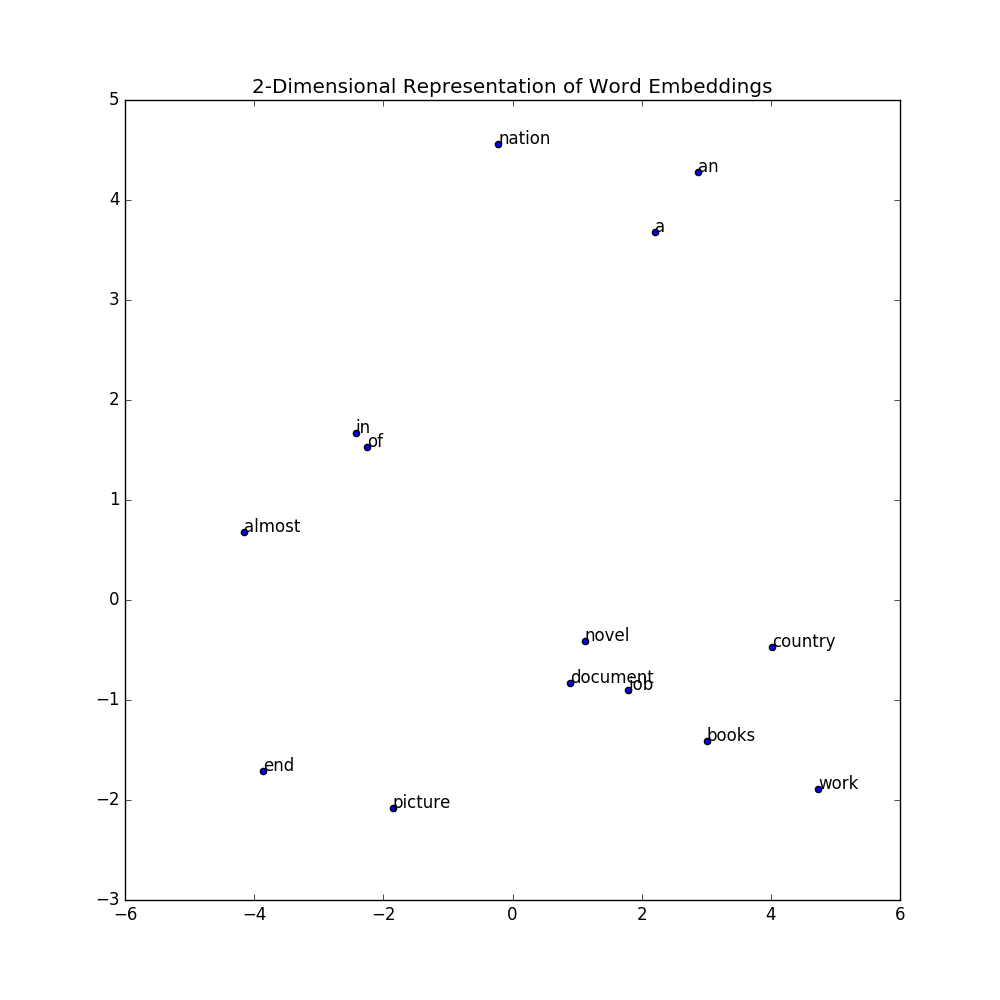
\includegraphics[width=10cm]{../plots/PTB_baseline_word_list_embeddings.png}
  \centering
  \caption{PTB Baseline Model: Embeddings of a selected word list}
  \label{fig:ptb1}
\end{figure}
These are reasonable embeddings: the tokens ``a" and ``an" are close to each other, as are ``novel", ``document' and ``books". However, we notice that ``nation" and ``country" are far apart, though they generally have similar meaning. We also notice that the pairs ``a" and ``an" (which are articles) and ``in" and `of" (which are prepositions) are far apart, even though they occupy a similar role in the English language, carrying limited meaning but generally used for syntactic correctness.
\newline
\newline
Next, we show embeddings of the same words according to our final model:

\begin{figure}[H]
  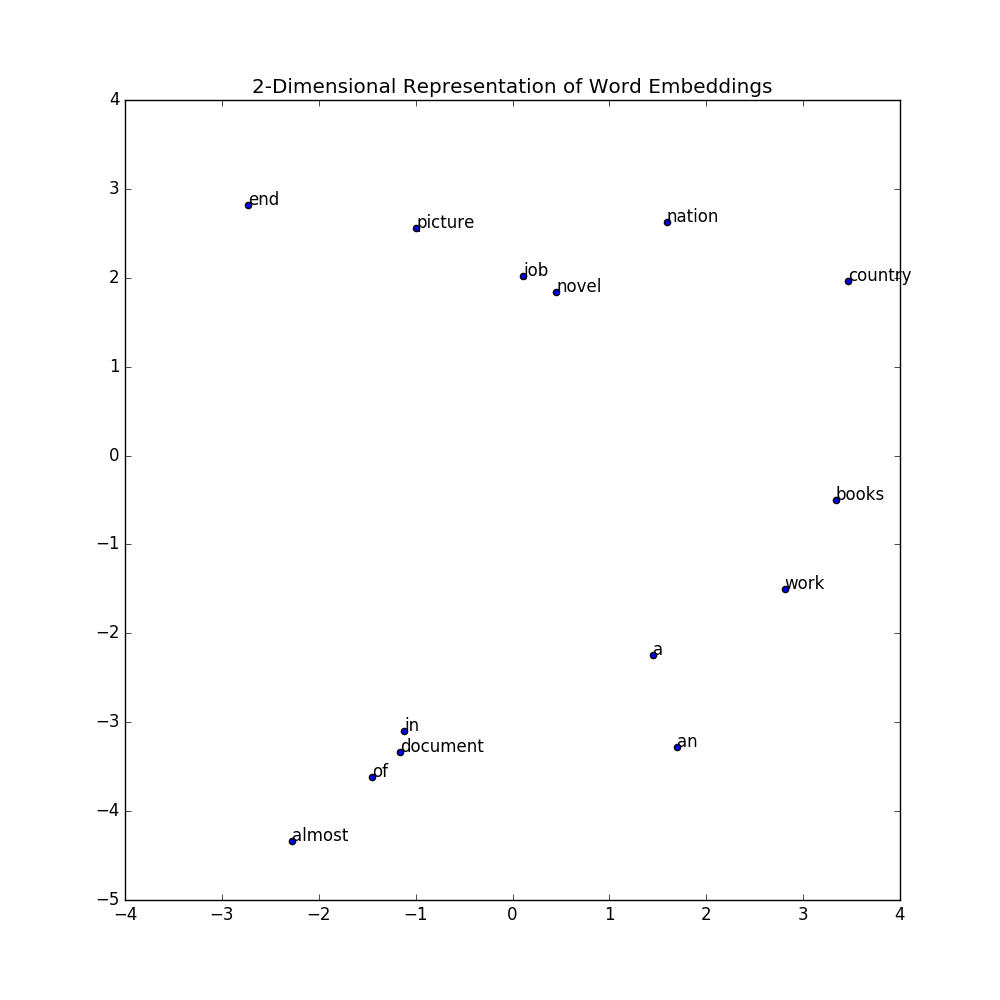
\includegraphics[width=10cm]{../plots/PTB_dropout_point3_two_layer_200_hidden_200_embeddding_word_list_embeddings.png}
  \centering
  \caption{PTB Final Model: Embeddings of a selected word list}
  \label{fig:ptb1}
\end{figure}
Though the list of selected words is small (for visual clarity), we can see that these embeddings are slightly better than those of the baseline. ``A" and ``an" are close together as are ``in" and ``of". Importantly, these pairs are slightly closer together than they were in the baseline embedding. ``Nation" and ``country" are much closer together. However, we note that even these embeddings are not uniformly superior: ``novel", ``document" and ``books" have floated apart. 
\newline
\newline
Next, to better understand our final model on the Gutenberg data, we again visualized the word embeddings in 2-d space using the t-SNE algorithm. As before, we generated a plot of selected word embeddings that would be informative, as well as another plot of random word embeddings.

\begin{figure}[H]
  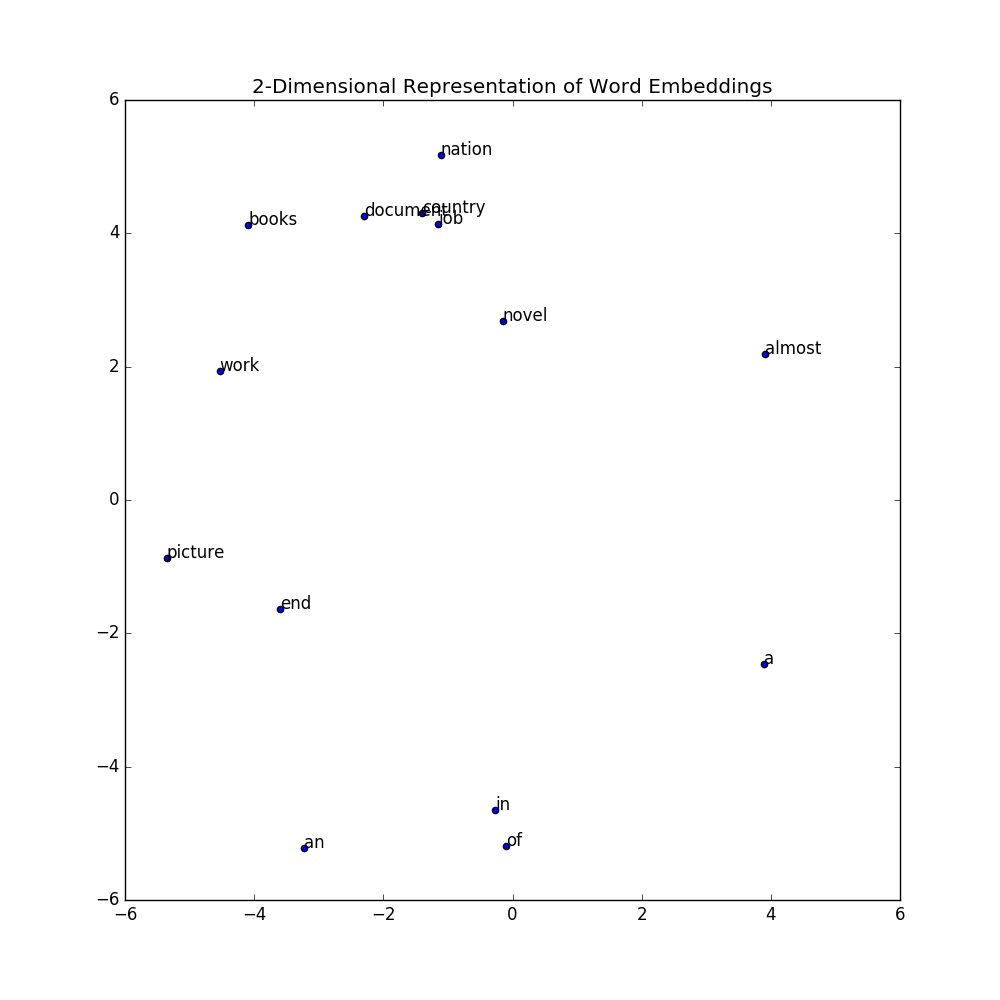
\includegraphics[width=10cm]{../plots/gutenberg_word_list_embeddings.png}
  \centering
  \caption{Gutenberg: Embeddings of a selected word list}
  \label{fig:boat1}
\end{figure}

\begin{figure}[H]
  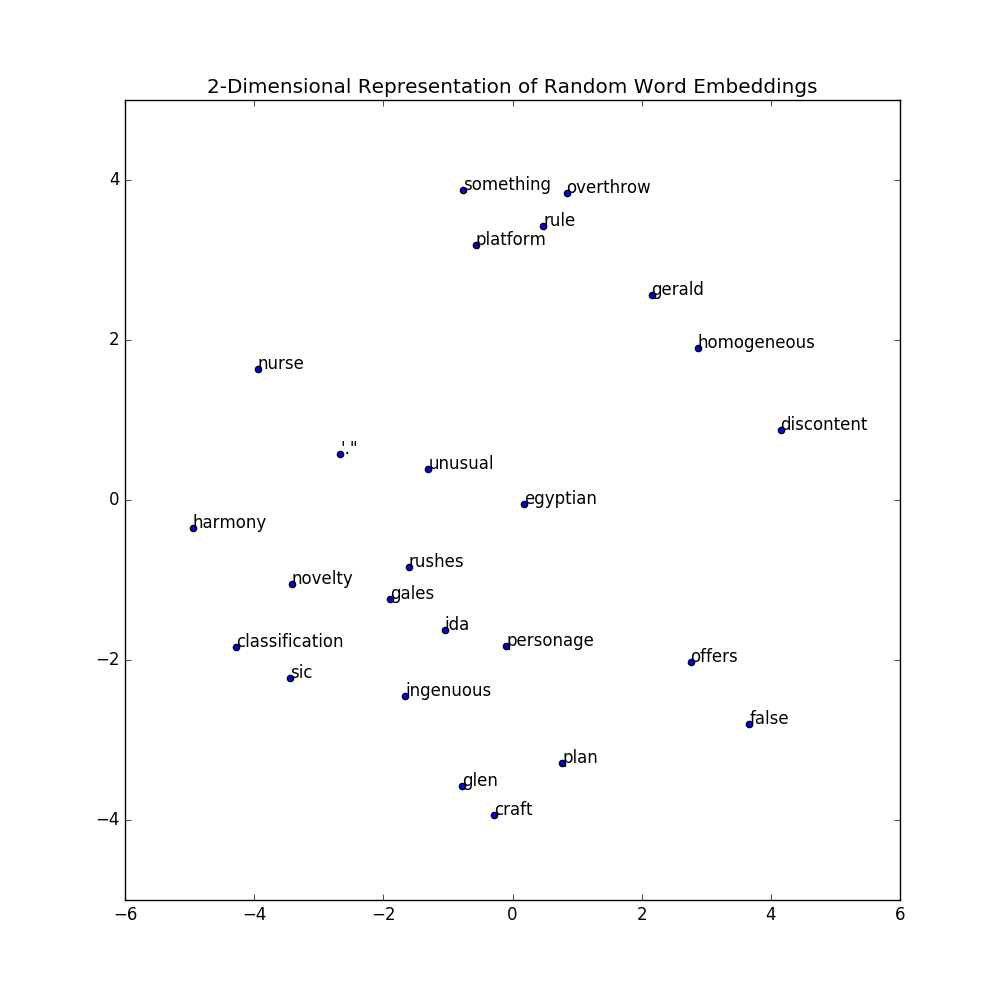
\includegraphics[width=10cm]{../plots/gutenberg_random_word_embeddings.png}
  \centering
  \caption{Gutenberg: Embeddings of a randomly selected words}
  \label{fig:boat1}
\end{figure}

In the selected word list plot, we can see that there are some relationships in language that are captured. 'nation' and 'country' are close, and 'documentary', 'books', and 'novel' are also close to each other. However, we would expect 'a' and 'an' to be very close to each other, and they are not in our embedding space. Also, 'job' is closer to 'country' and 'documentary' than it is to 'work', although part-of-speech may be playing a part here as the first 3 are all nouns while 'work' more commonly appears as a verb than a noun. 
\newline
\newline
In the plot of random word embeddings, it is quite hard to assess whether the model is learning well or not. It seems that a random selection of words populate the space rather evenly and since no two words are very close in meaning, it is hard to assess the model. However, we can see that 'overthrow' and 'rule' are close to each other, and they are often used in similar contexts even though they have somewhat opposite meanings.
\newline
\newline
In general, it seems that our model has learned some of the relationships and dependencies in language but there is still room for improvement. With more time and computing power, we would have liked to try training a deeper model (3+ layers) with more of the training data and possibly larger embedding and hidden state sizes to see if a more powerful model can be trained.  
\end{document}
